\chapter{Drupal theming}

In this chapter we are going to learn how to change the look of our site. First we will learn how to change the basic theme settings. Next you will learn how to install a custom theme. The last part of this chapter explains how to extend a theme and add your own html and css.

\section{Theme basics}

\subsection{Changing the theme settings}

To view the settings of your current theme (Bartik) go to \textbf{Appearance $\rightarrow$ Settings}. On his page you can see a tab for each of the enabled themes (Figure \ref{fig:theme_settings_enabled_themes}).

\begin{figure}[H]
	\centering
	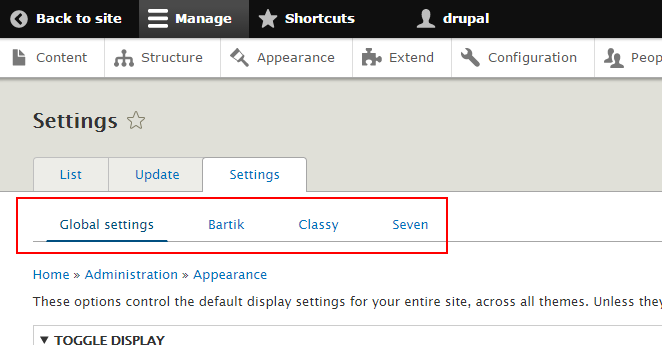
\includegraphics[width=\textwidth]{chapter10/theme_settings_enabled_themes}
	\caption{Theme settings, overview enabled themes.}
	\label{fig:theme_settings_enabled_themes}
\end{figure}

Some themes will come with more settings, such as colour options. Compare the themes you have enabled. Many theme specific settings are very similar to the global settings. When you change settings per theme, they will override the Global settings for that theme. Some of the more interesting themes will offer much more functionality. The default Bartik theme implements functionality from the Colour module, play around with them a little. The Colour module can, but does not have to be implemented in a theme, so not
every theme will offer this functionality.

\begin{figure}[H]
	\centering
	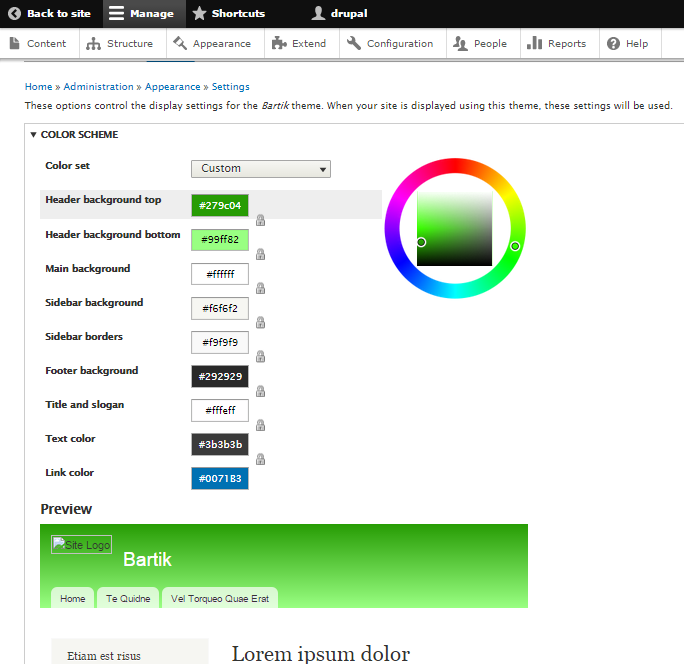
\includegraphics[width=\textwidth]{chapter10/bartik_color_settings}
	\caption{Changing the Bartik color settings.}
	\label{fig:bartik_color_settings}
\end{figure}

Notice in figure \ref{fig:bartik_color_settings} the logo image is not displayed. This is because we are using a custom logo image.

\subsection{Installing a new theme}

In Drupal there are several ways to install a theme. The fist option is to go to \textbf{Appearance $\rightarrow$ Install new theme}. 

\begin{figure}[H]
	\centering
	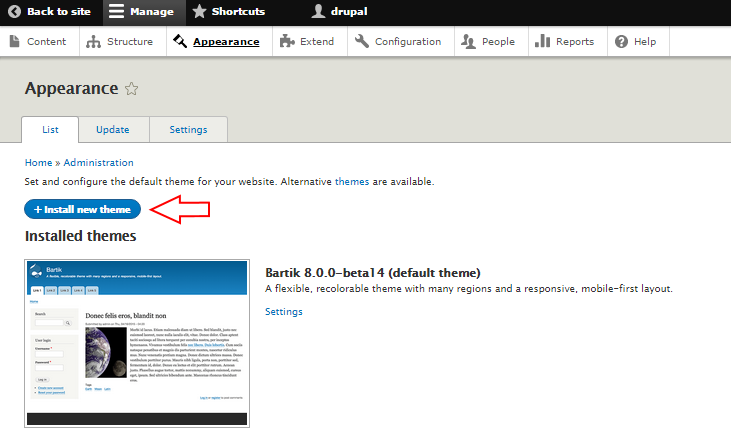
\includegraphics[width=\textwidth]{chapter10/install_new_theme_button}
	\caption{Click the button to install a new theme.}
	\label{fig:install_new_theme_button}
\end{figure}

This will take you to a page where you can either install from a URL, or upload an archive from your local computer.

\begin{figure}[H]
	\centering
	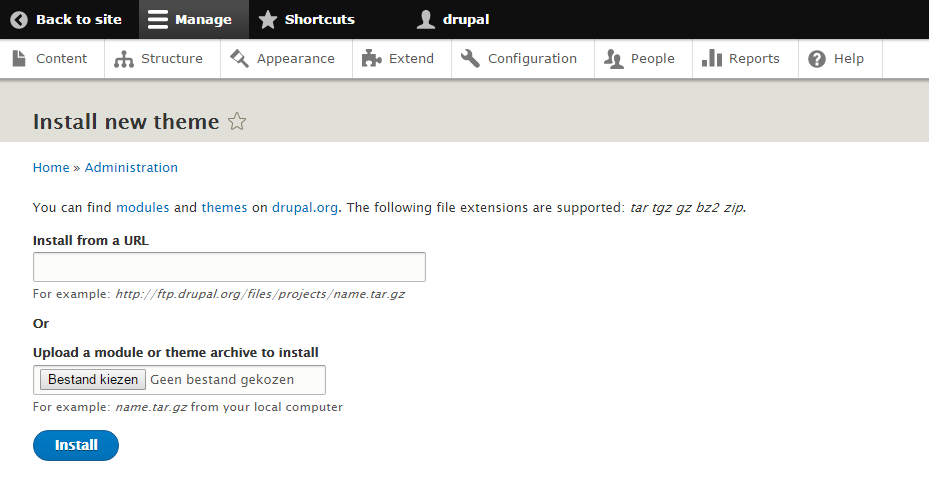
\includegraphics[width=\textwidth]{chapter10/install_new_theme_page}
	\caption{On this page you can choose to install a theme by copying the url from the location where the theme is hosted or uploading the theme from your local computer.}
	\label{fig:install_new_theme_page}
\end{figure}

Either way, you will have to visit the theme project page at \url{https://drupal.org/project/theme_name} and find the file URL for the archive, or just download it, which takes us to option number two.\\

The second way to install a new theme downloading it, unpacking it and placing it in the appropriate folder, which is \url{/themes} (Figure \ref{fig:theme_install_location}). 

\begin{figure}[H]
	\centering
	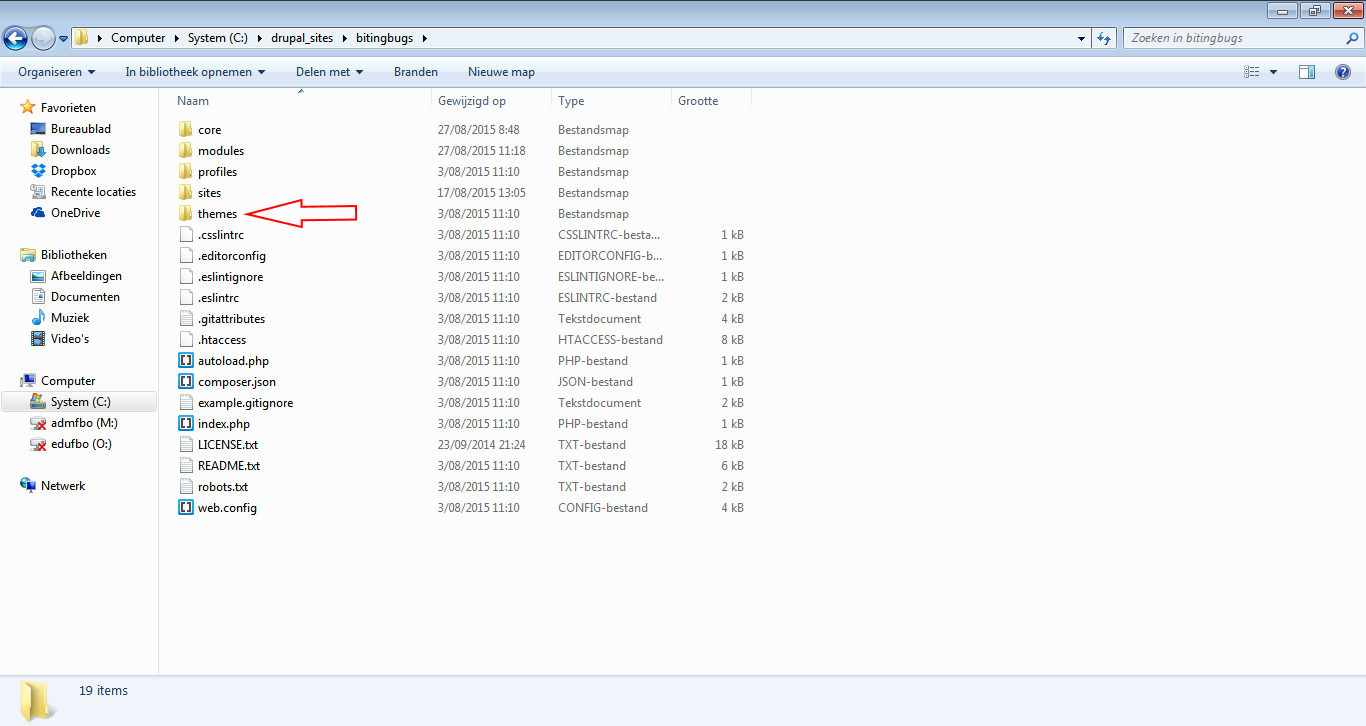
\includegraphics[width=\textwidth]{chapter10/theme_install_location}
	\caption{Theme install location.}
	\label{fig:theme_install_location}
\end{figure}

The third and quickest way to install a theme is through the Drush command line tool. Using Drush we have to type the following two commands:

\begin{lstlisting}[language=bash]
drush dl theme_name
drush en theme_name
\end{lstlisting}

The theme\_name, or module\_name in case you are installing modules, should be the machine name. This can be found in the URL of the project page on drupal.org, it is the word after project/. For example in \url{www.drupal.org/project/bartik} the machine name is \textbf{bartik}.

Drupal 8 has all core code and themes under a directory named /core. For contributed and custom themes drupal uses the /themes folder that lives on the same level as the /core folder. For people having experience with drupal 7 themes, these are the 2 most apparent changes when we look at a theme folder:
\begin{itemize}
	\item The *.infofile changes to *.info.yml.
	\item The *.tpl.phpfiles change to *.html.twig.
\end{itemize}
● 
